\section{Komponenten}
\textcolor{blue}{\textit{Es sollen die in der Architektur definierten Komponenten weiter beschrieben werden. Dazu ist ihre innere Struktur zu beschreiben und mit Hilfe von Klassendiagrammen, Kompositionsstrukturdiagrammen sowie Komponentendiagrammen zu modellieren. Pro Komponente sollen Parts, Ports und Konnektoren beschrieben werden. Pro Komponente sollen Klassen und Assoziationen sowie deren Methoden und Attribute definiert werden, die für die Durchführung der vorher beschriebenen Abläufe innerhalb der Komponenten benötigt werden. In den Klassendiagrammen müssen sich gegebenenfalls die in Abschnitt 4 definierten Schnittstellen wiederfinden.\\\\
Komponenten können sich während der Ausführung in verschiedenen Zuständen befinden. Sie wechseln diese, ausgelöst durch interne oder externe Ereignisse. Zustandsbezogenes Verhalten wird durch Zustandsdiagramme modelliert. Auslösende Ereignisse müssen als Operationen an den Komponentenschnittstellen zur Verfügung stehen. Ebenso sollen durch Transitionen ausgelöste Aktionen in der Komponente oder an externen Komponenten verfügbar sein.\\\\
Es muss nicht für jede Komponente ein Zustandsdiagramm erstellt werden. Zustandsdiagramme sollen nur für die Komponenten modelliert werden, die reaktiven Charakter haben und in verschiedenen Modi operieren.\\
}}

\begin{figure}[H]
\centering
\includegraphics[width=0.75\textwidth]{img/Komponenten1.png}
\caption{\textcolor{blue}{Durch eigene Diagramm ersetzen}}
\label{KomponentenStruktur1}
\end{figure}

\begin{figure}[H]
\centering
\includegraphics[width=0.85\textwidth]{img/Komponenten2.png}
\caption{\textcolor{blue}{Durch eigene Diagramm ersetzen}}
\label{KomponentenStruktur2}
\end{figure}

\begin{figure}[H]
\centering
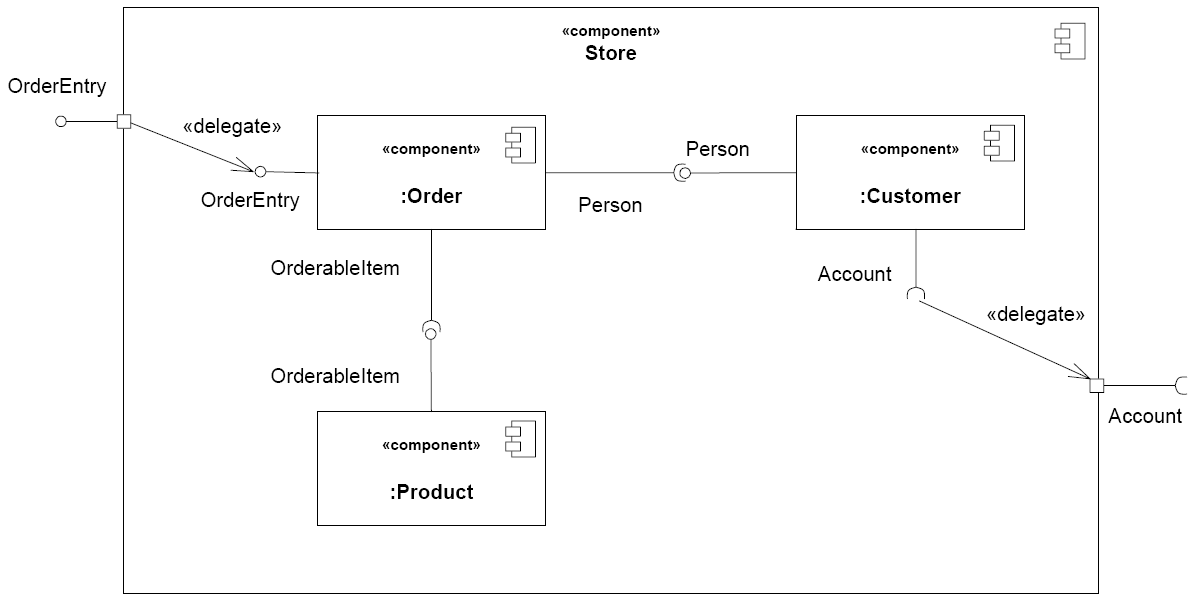
\includegraphics[width=1\textwidth]{img/Komponenten3.png}
\caption{\textcolor{blue}{Durch eigene Diagramm ersetzen}}
\label{KomponentenStruktur3}
\end{figure}

\begin{figure}[H]
\centering

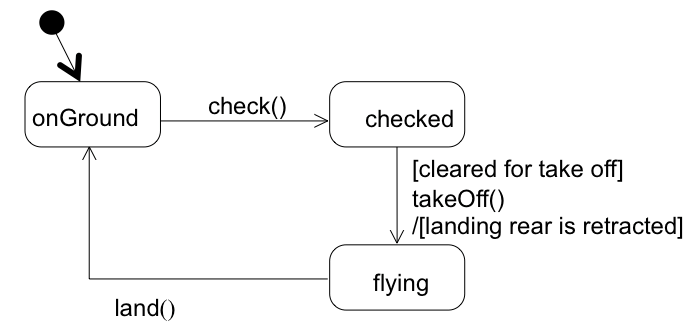
\includegraphics[width=0.6\textwidth]{img/Komponenten4.png}
\caption{\textcolor{blue}{Durch eigene Diagramm ersetzen}}
\label{KomponentenStruktur4}
\end{figure}